% The weight 3+4\cos\phi+\cos 2\phi = 2(1+\cos\phi)^2 on [0,2\pi].
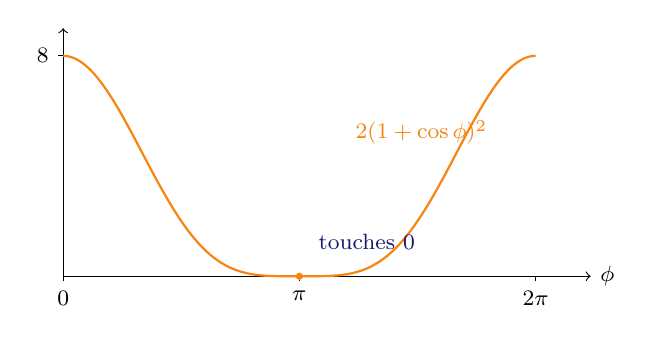
\begin{tikzpicture}[every node/.style={font=\footnotesize}]
  \draw[->] (0,0)--(6.7,0) node[right] {$\phi$};
  \draw[->] (0,0)--(0,3.15);
  \draw[BurntOrange,thick] plot[domain=0:360,samples=91] ({6*\x/360},{2.8*(1+cos(\x))*(1+cos(\x))/4});
  \draw (0,0)--(0,-0.06) node[below] {$0$};
  \draw (3,0)--(3,-0.06) node[below] {$\pi$};
  \draw (6,0)--(6,-0.06) node[below] {$2\pi$};
  \draw (0,2.8)--(-0.06,2.8) node[left] {$8$};
  \fill[BurntOrange] (3,0) circle (1.3pt);
  \node[BurntOrange,above] at (4.55,1.55) {$2(1+\cos\phi)^2$};
  \node[MidnightBlue,above right] at (3.12,0.22) {touches $0$};
\end{tikzpicture}
